\documentclass[a4paper,12pt]{article} 

%%% Работа с русским языком
\usepackage{cmap}                           % поиск в PDF
\usepackage{mathtext} 			 	       % русские буквы в формулах
\usepackage[T2A]{fontenc}               % кодировка
\usepackage[utf8]{inputenc}              % кодировка исходного текста
\usepackage{siunitx}
\usepackage[english,russian]{babel}  % локализация и переносы
\usepackage[left=2cm,right=2cm,
    top=2cm,bottom=3cm,bindingoffset=0cm]{geometry}
\usepackage{wrapfig}
\usepackage{gensymb}
\usepackage{textcomp}
\usepackage{multirow}
\usepackage{pgfplots}
\usepackage{amsmath,amsfonts,amssymb,amsthm,mathtools} % AMS
\usepackage{euscript}	 % Шрифт Евклид
\usepackage{mathrsfs} % Красивый матшрифт
\usepackage{graphicx}%Вставка картинок правильная
\usepackage{float}%"Плавающие" картинки
\usepackage{wrapfig}%Обтекание фигур (таблиц, картинок и прочего)
\title{Лабораторная работа 5.5

Компьютерная сцинтилляционная $\gamma$-спектрометрия}
\author{Кагарманов Радмир Б01-102}
\date{18 декабря 2023 г.}

\begin{document}
\maketitle
\thispagestyle{empty}
\newpage
\setcounter{page}{1}

\paragraph{Цель работы:}исследовать сцинтилляционные гамма-спектрометры на основе неорганического кристалла NaI(Tl).

\paragraph{Теория\\}
Основными процессами взаимодействия гамма-излучения с веществом
являются фотоэффект, эффект Комптона и образование электрон-позитронных пар. Каждый из этих процессов вносит свой
вклад в образование наблюдаемого спектра. \par
Фотоэффект - процесс взаимодействия гамма-кванта с электроном, связанным с атомом, при котором электрону передается вся энергия гамма-кванта. Фотоэффект особенно существенен для тяжелых веществ, где он идет с заметной вероятностью даже при высоких энергиях гамма-квантов. В легких
веществах фотоэффект становится заметен лишь при относительно небольших энергиях гамма-квантов.\par

Эффект Комптона - упругое рассеяние фотона на свободном электроне,
сопровождающееся изменением длины волны фотона (реально этот процесс
происходит на слабо связанных с атомом внешних электронах). Максимальная энергия образующихся комптоновских электронов соответствует рассеянию гамма-квантов на 180о
и равна\par

При достаточно высокой энергии гамма-кванта наряду с фотоэффектом и эффектом Комптона
может происходить третий вид взаимодействия гамма-квантов с веществом –
образование электрон-позитронных пар. Процесс образования пар не может
происходить в пустоте, так как в этом случае не выполняются совместно
законы сохранения энергии и импульса. В присутствии ядра или электрона
процесс образования пары гамма-квантом возможен, так как можно распределить энергию и импульс гамма-кванта между тремя частицами без противоречия с законами сохранения. При этом если процесс образования пары
идет в кулоновском поле ядра, то энергия образующегося ядра отдачи оказывается весьма малой, так что пороговая энергия гамма-кванта $E_{пор}$, необходимая для образования пары, практически совпадает с удвоенной энергией
покоя электрона $2mc^2=1,022$ МэВ. \par
Появившиеся в результате процесса образования пар частицы теряют
свою кинетическую энергию на ионизацию среды. Таким образом, вся энергия электрона остается в детекторе. Позитрон будет двигаться до тех пор,
пока практически не остановится, а затем аннигилирует с электроном среды,
в результате чего появятся два гамма-кванта. Т.е., кинетическая энергия
позитрона также останется в детекторе. Далее возможны три варианта развития событий:\par
а) оба родившихся гамма-кванта не вылетают из детектора, и тогда вся
энергия первичного гамма-кванта останется в детекторе, а в спектре появится
пик с $E=E_{\gamma}$;\par
б) один из родившихся гамма-квантов покидает детектор, и в спектре появляется пик, соответствующий энергии $E=E_{\gamma} - E_0$, где $E_0 = mc^2 = 511$ кэВ;\par
в) оба родившихся гамма-кванта покидают детектор, и в спектре появляется пик, соответствующий энергии $E=E_{\gamma} - 2E_0$.\par
Таким образом, любой спектр, получаемый с помощью гаммаспектрометра, описывается несколькими компонентами, каждая из которых
связана с определенным физическим процессом. Каждый процесс взаимодействия гамма-квантов с веществом (фотоэффект, эффект Комптона и образование электрон-позитронных пар) вносит свой вклад в образование спектра.\par
Энергетическим разрешением спектрометра называется величина:
\begin{equation}
    R_i=\frac{\Delta E_i}{E_i}
\end{equation}
\paragraph{Экспериментальная установка\\}
\begin{figure}[!h]
\centering
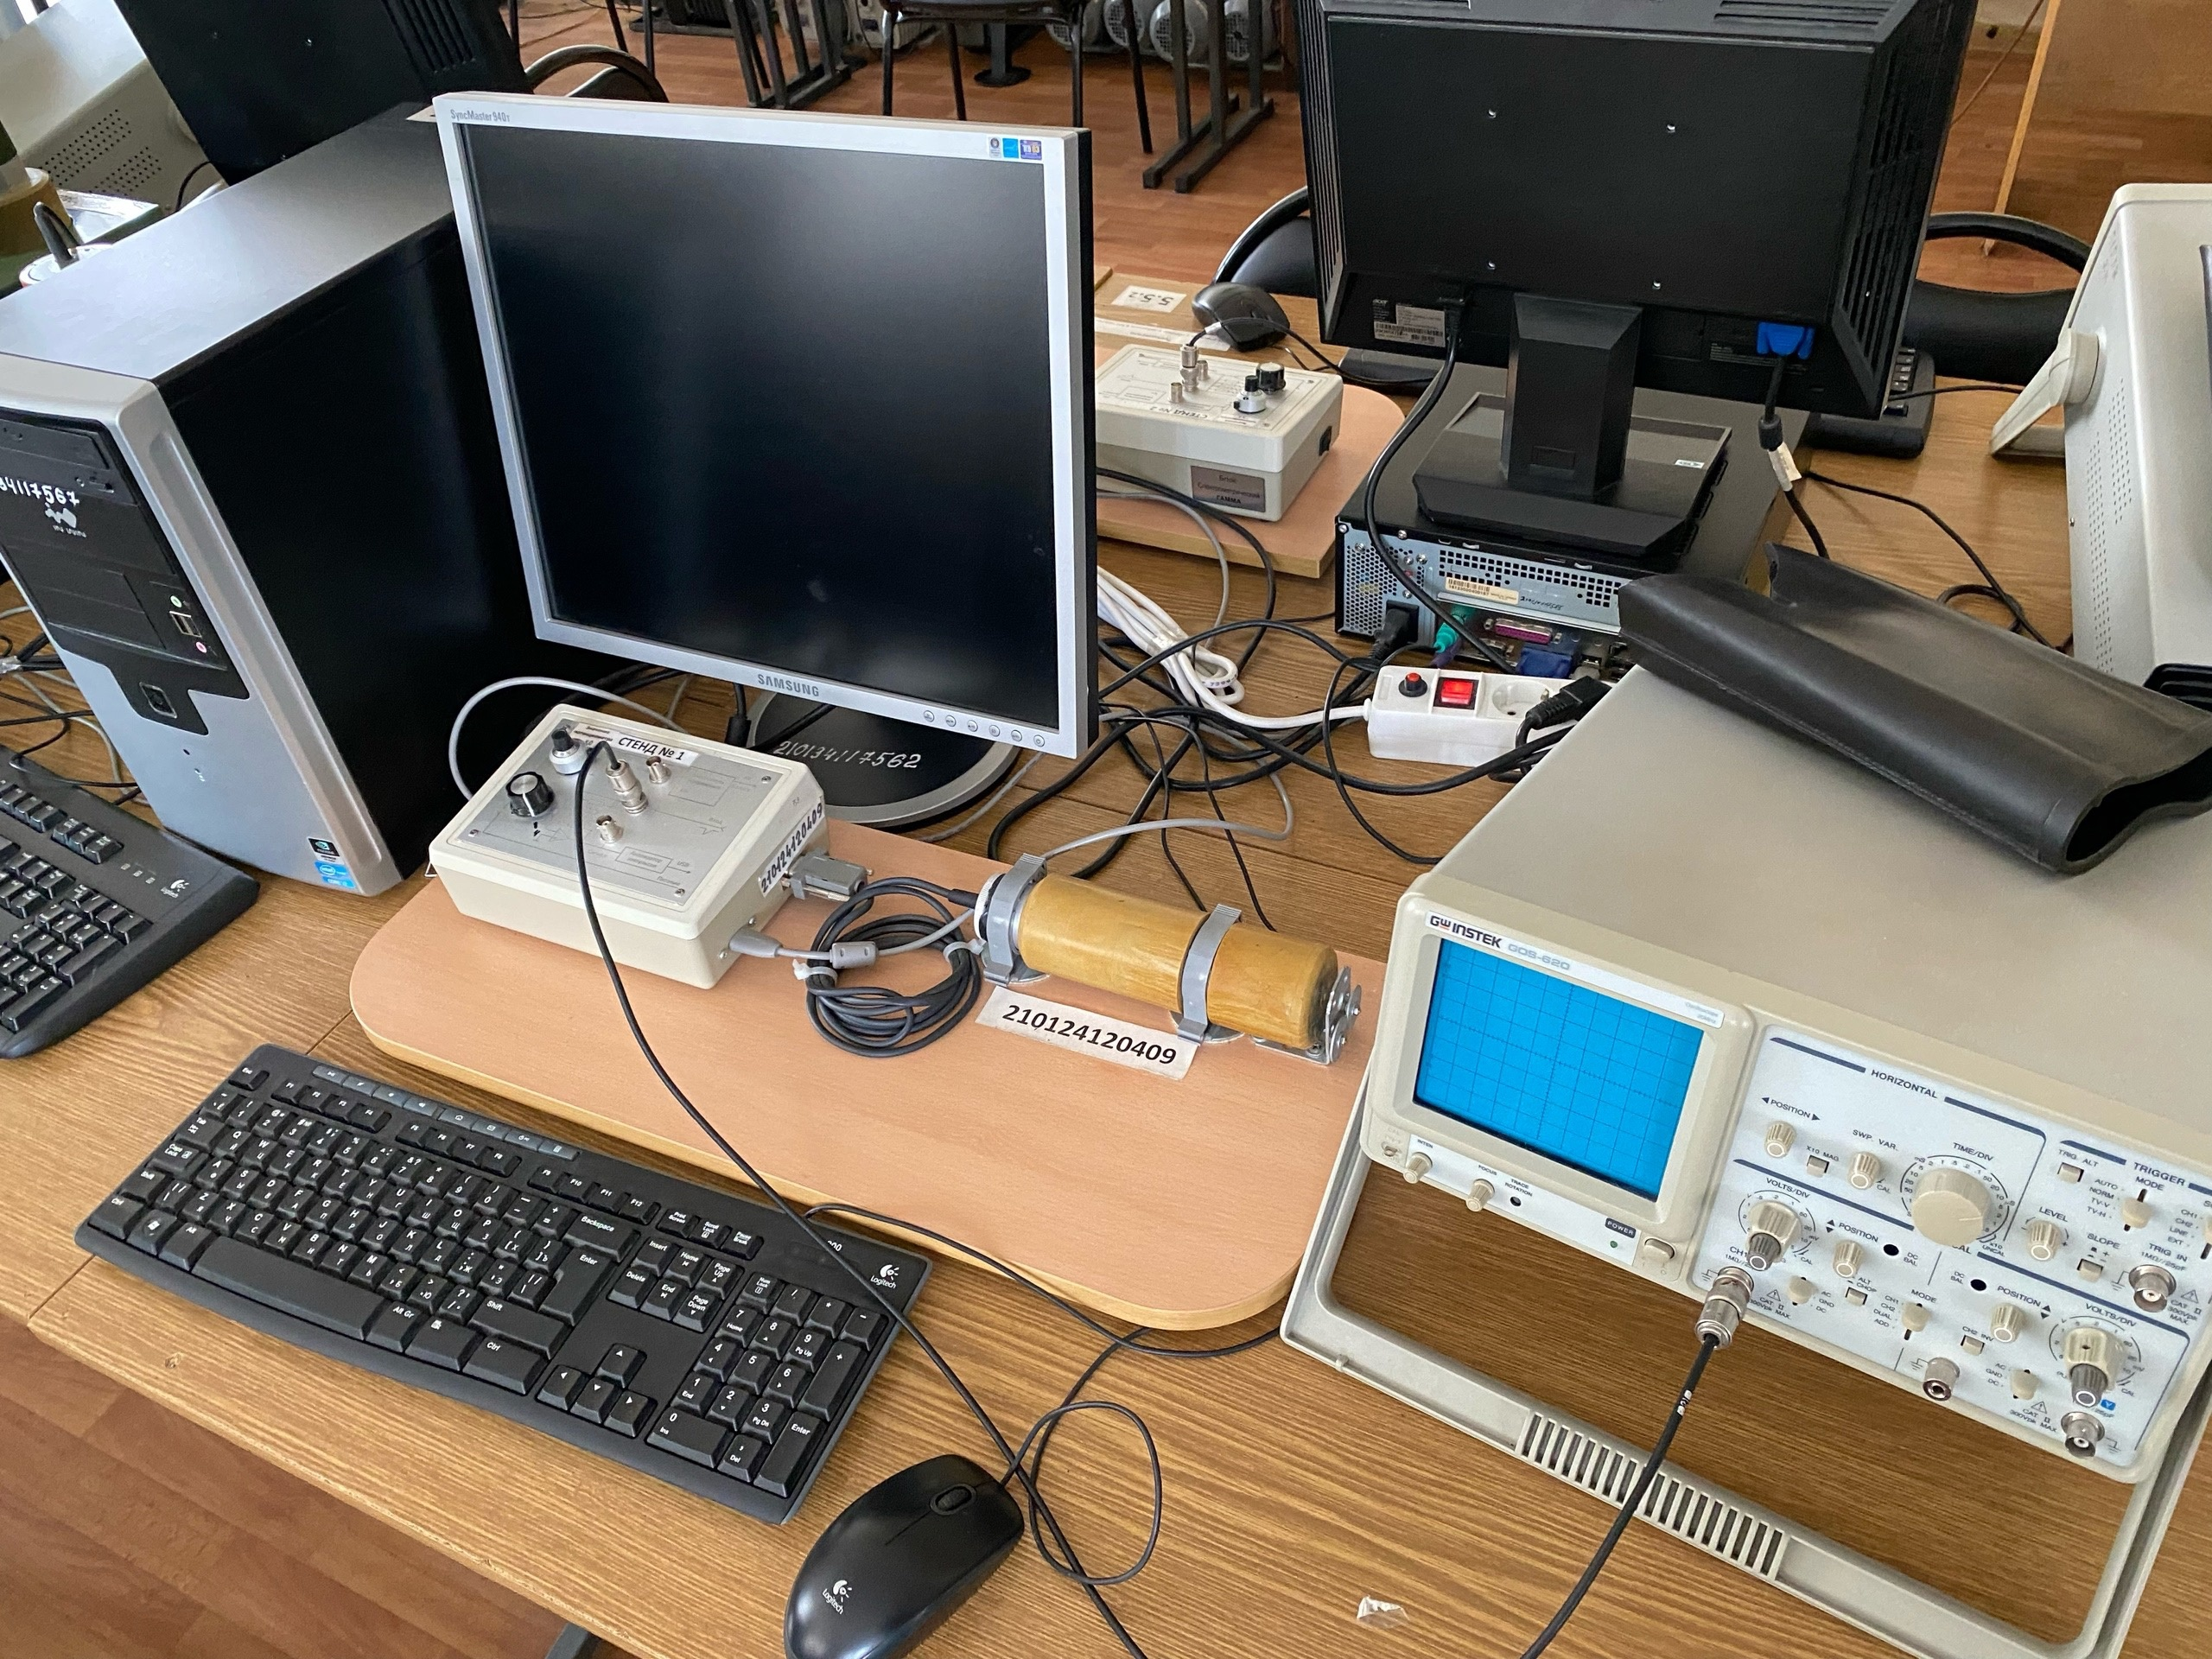
\includegraphics[width=0.8\linewidth]{экспериментальная.jpg}
\caption{Экспериментальная установка}
\label{fig:mpr}
\end{figure}
В данной работе использовались сцинтиллятор, ФЭУ, высоковольтный блок питания для ФЭУ, компьютер для сбора данных и их обработки.

\paragraph{Обработка результатов:}
\subparagraph{1.} 
\begin{center}
\begin{tabular}{|c|c|c|c|c|c|}
\hline
Источник & $N_{i}$ & $\Delta N_{i}$ & $E_i, $ МэВ & $\Delta E_{i}$, МэВ & $R_{i}$ \\ \hline
$^{60}Co$ & 1150 & 60 & 0,154 & 0,008 &
0,052 \\ \hline
$^{22}Na$ & 465 & 40 & 0,062 & 0,005 & 0,081 \\ \hline
$^{137}Cs$ & 590 & 40 & 0,079 & 0,005 & 0,063 \\ \hline
\end{tabular}\\
\end{center}

\subparagraph{2.} Построим по полученным данным график зависимости $R^2=f(1/E_i)$, чтобы проверить зависимость $R=\frac{\Delta E_i}{E_i}=\frac{const}{\sqrt{E_i}}$. Видно, что точки не лежат на одной прямой.

\begin{figure}[!h]
\centering
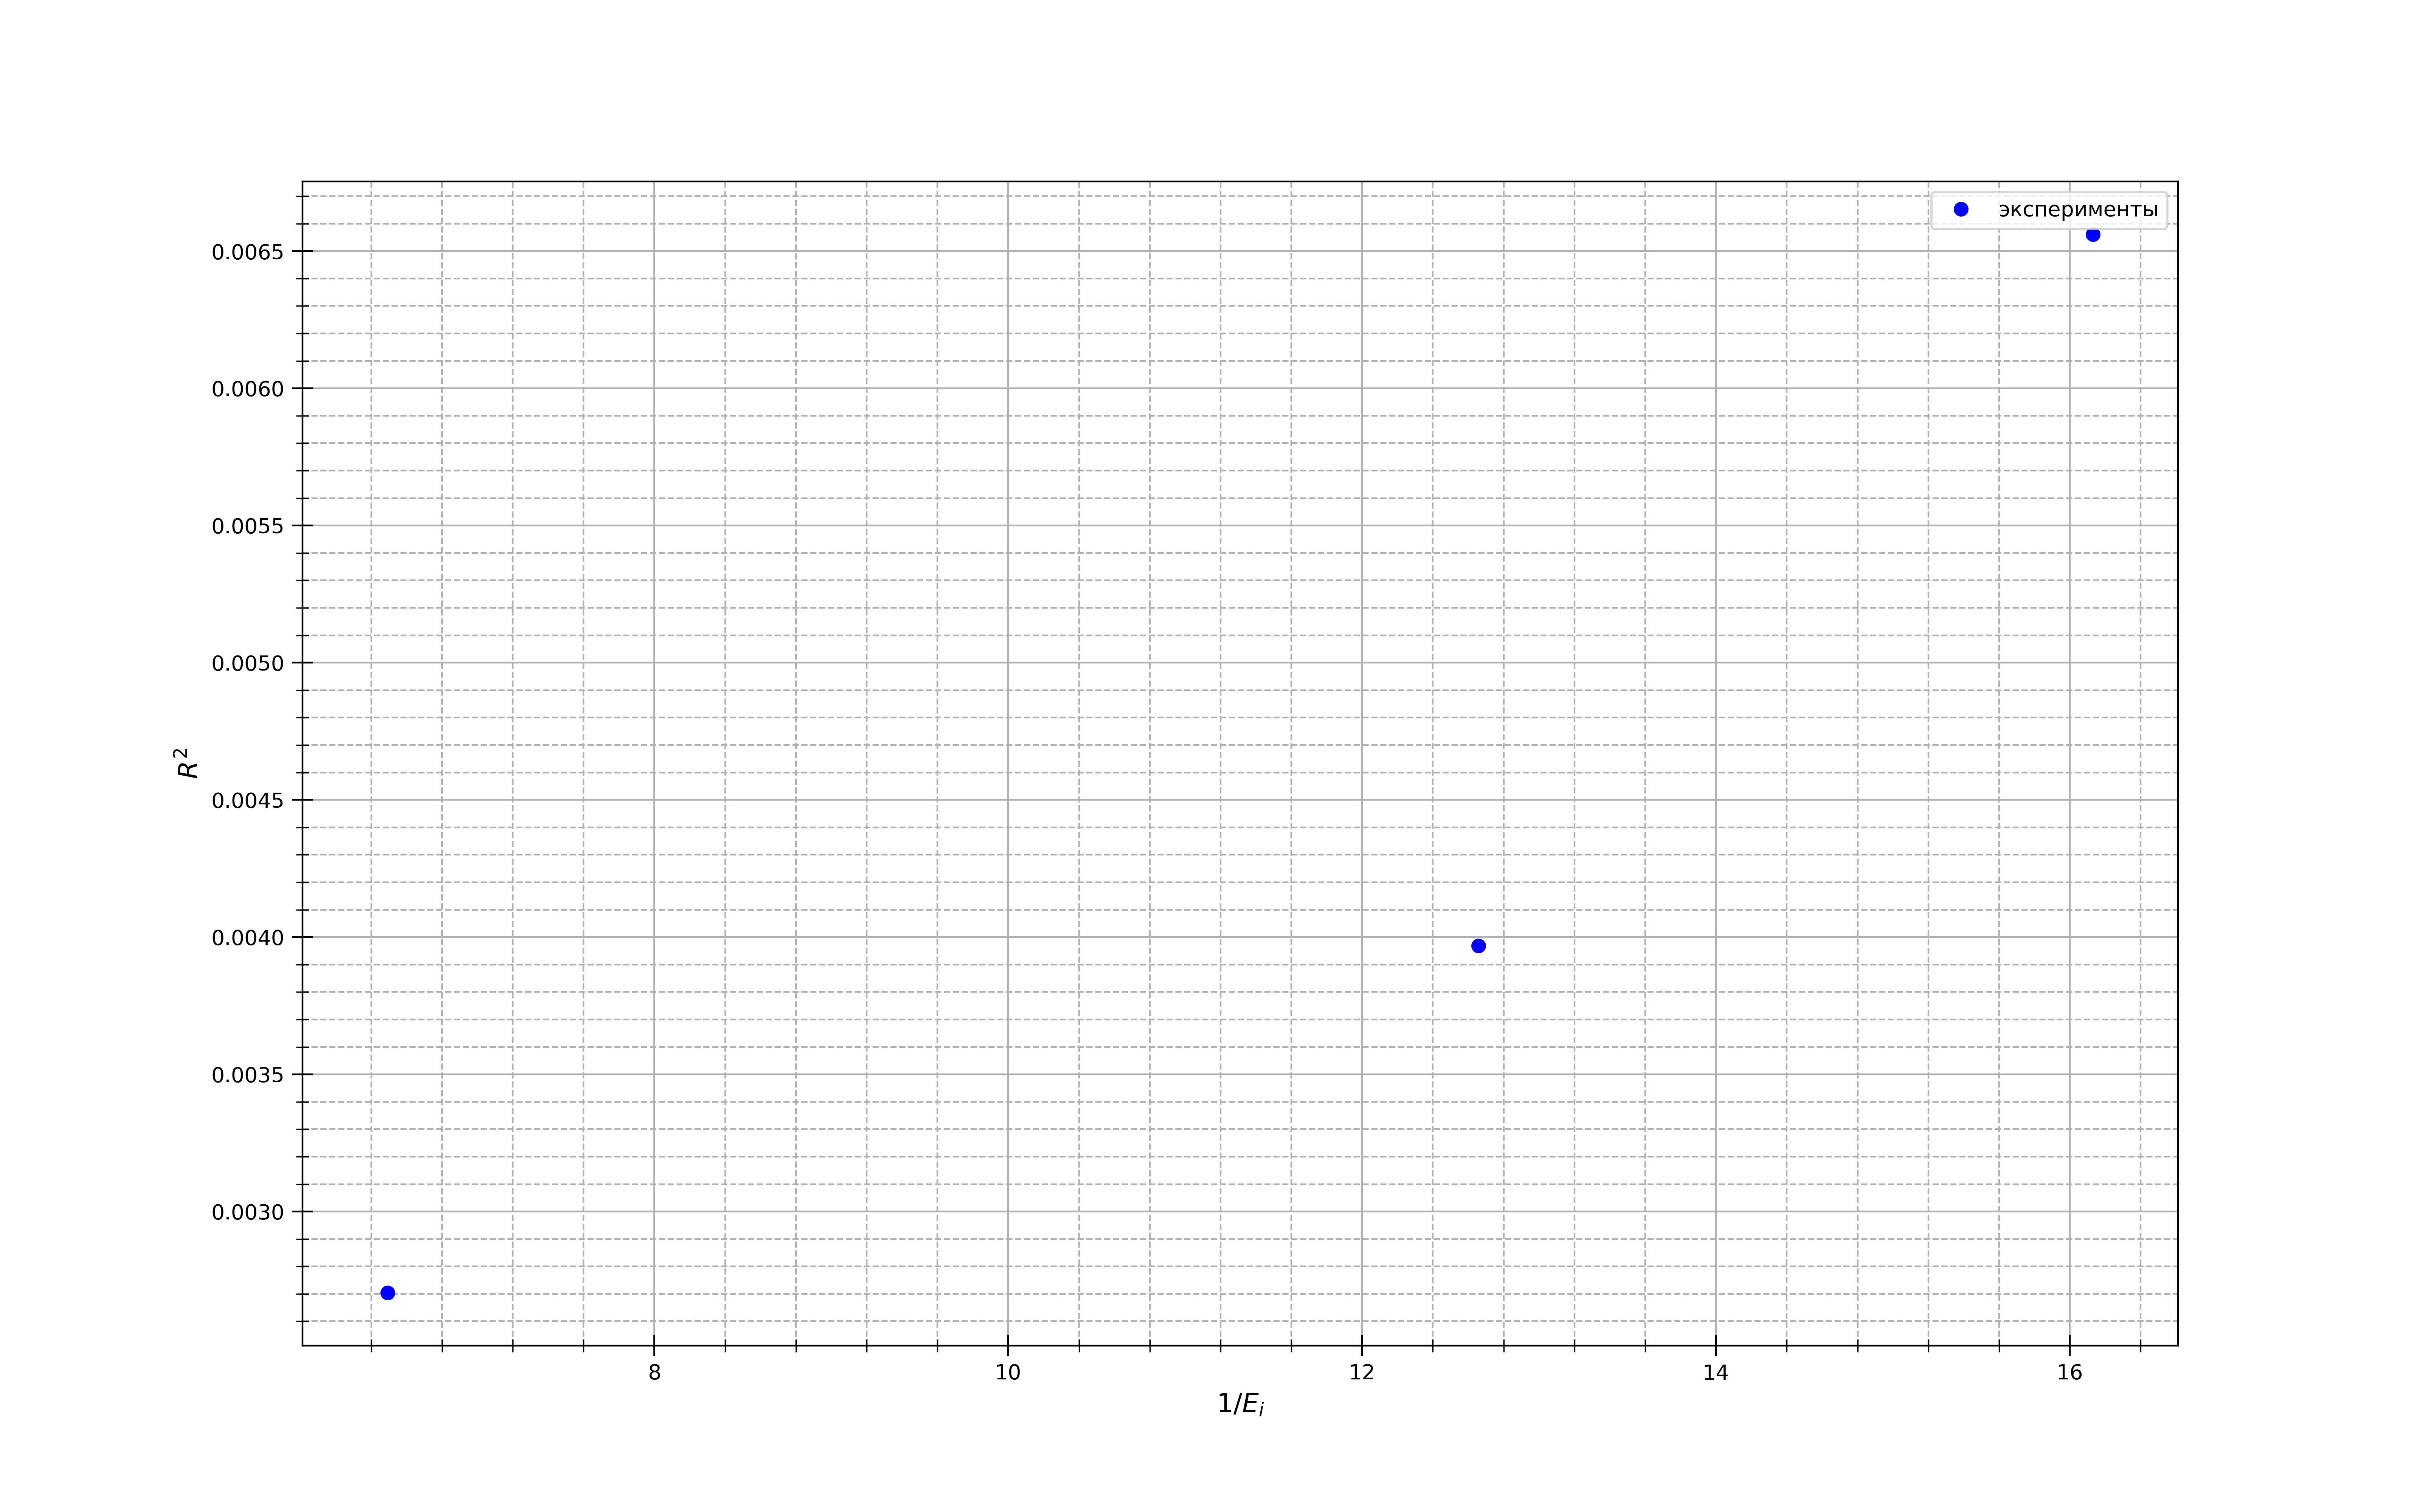
\includegraphics[width=0.8\linewidth]{R^2.png}
\caption{$R^2=f(1/E_i)$}
\label{fig:mpr}
\end{figure}

\newpage
\subparagraph{3.} Построим график зависимости энергии пика обратного рассеяния от энергии фотопика.

\begin{figure}[!h]
\centering
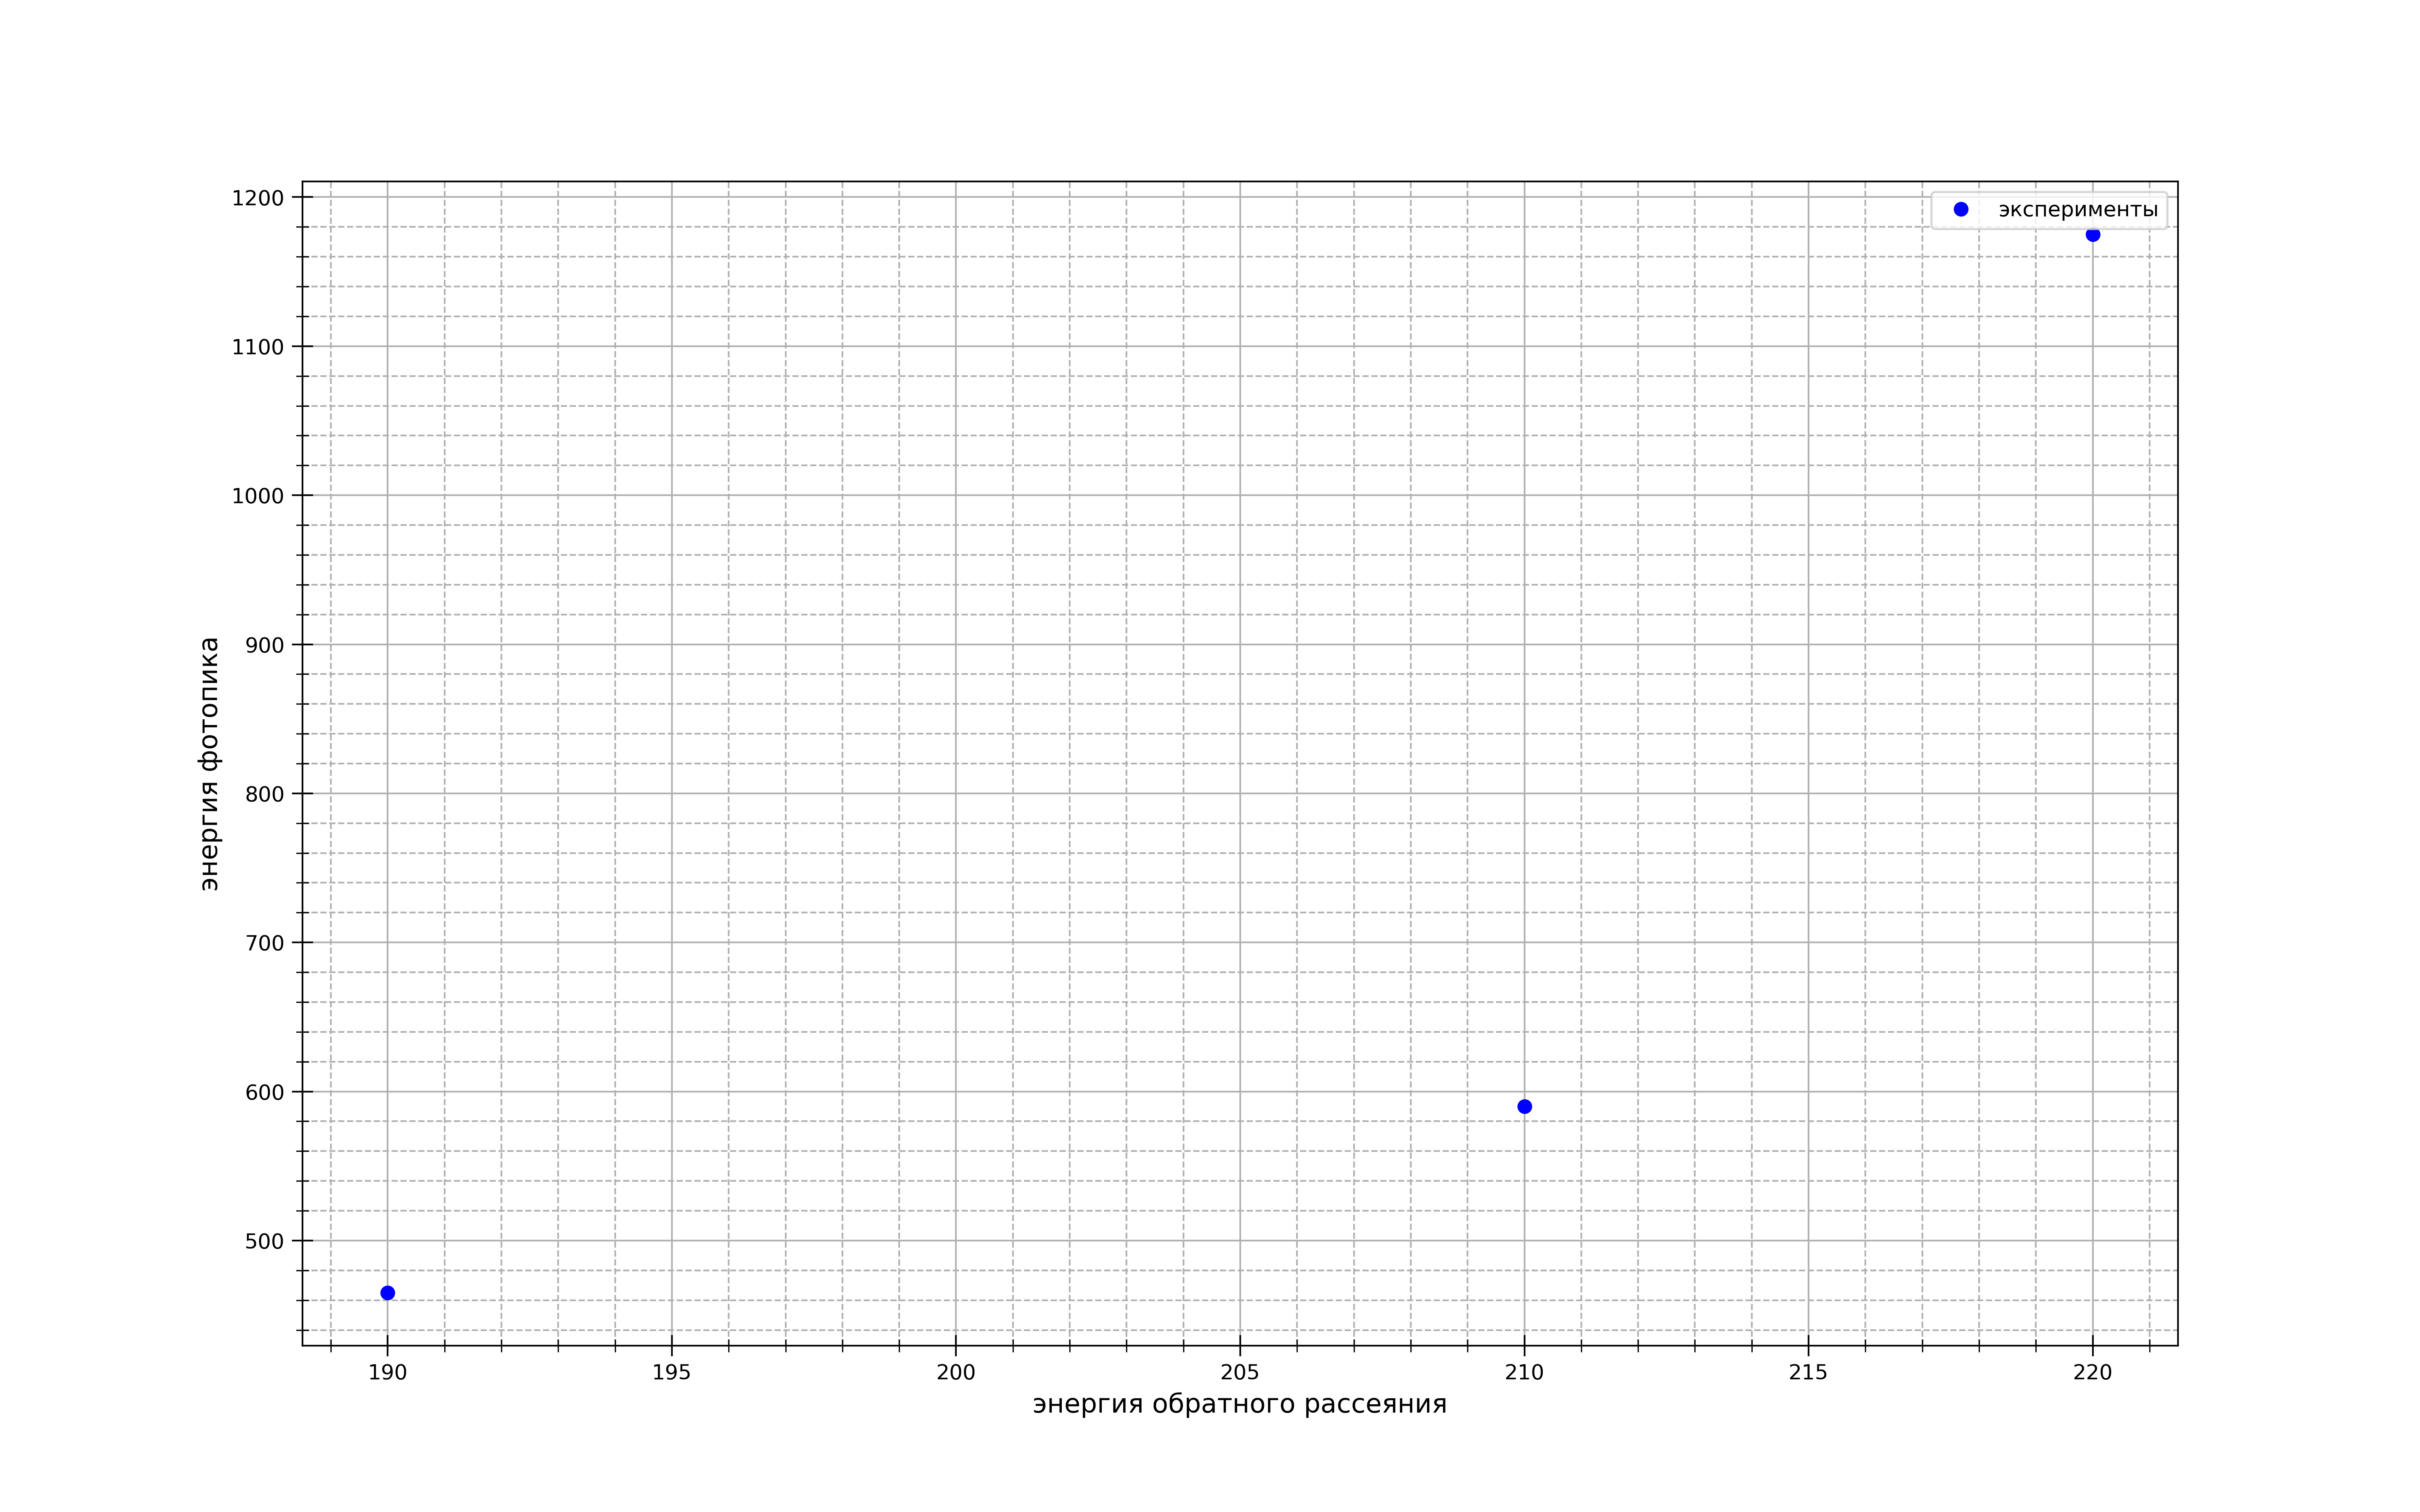
\includegraphics[width=0.8\linewidth]{piki.png}
\caption{График зависимости энергии пика обратного рассеяния от энергии фотопика}
\label{fig:mpr}
\end{figure}
\paragraph{Вывод:}В данной лабораторной работе мы исследовали спектры для $^{137}Cs$, $^{22}Na$, $^{60}Co$. Нашли для них энергии пиков полного поглощения и разрешающую способность.

\begin{figure}[!h]
\centering
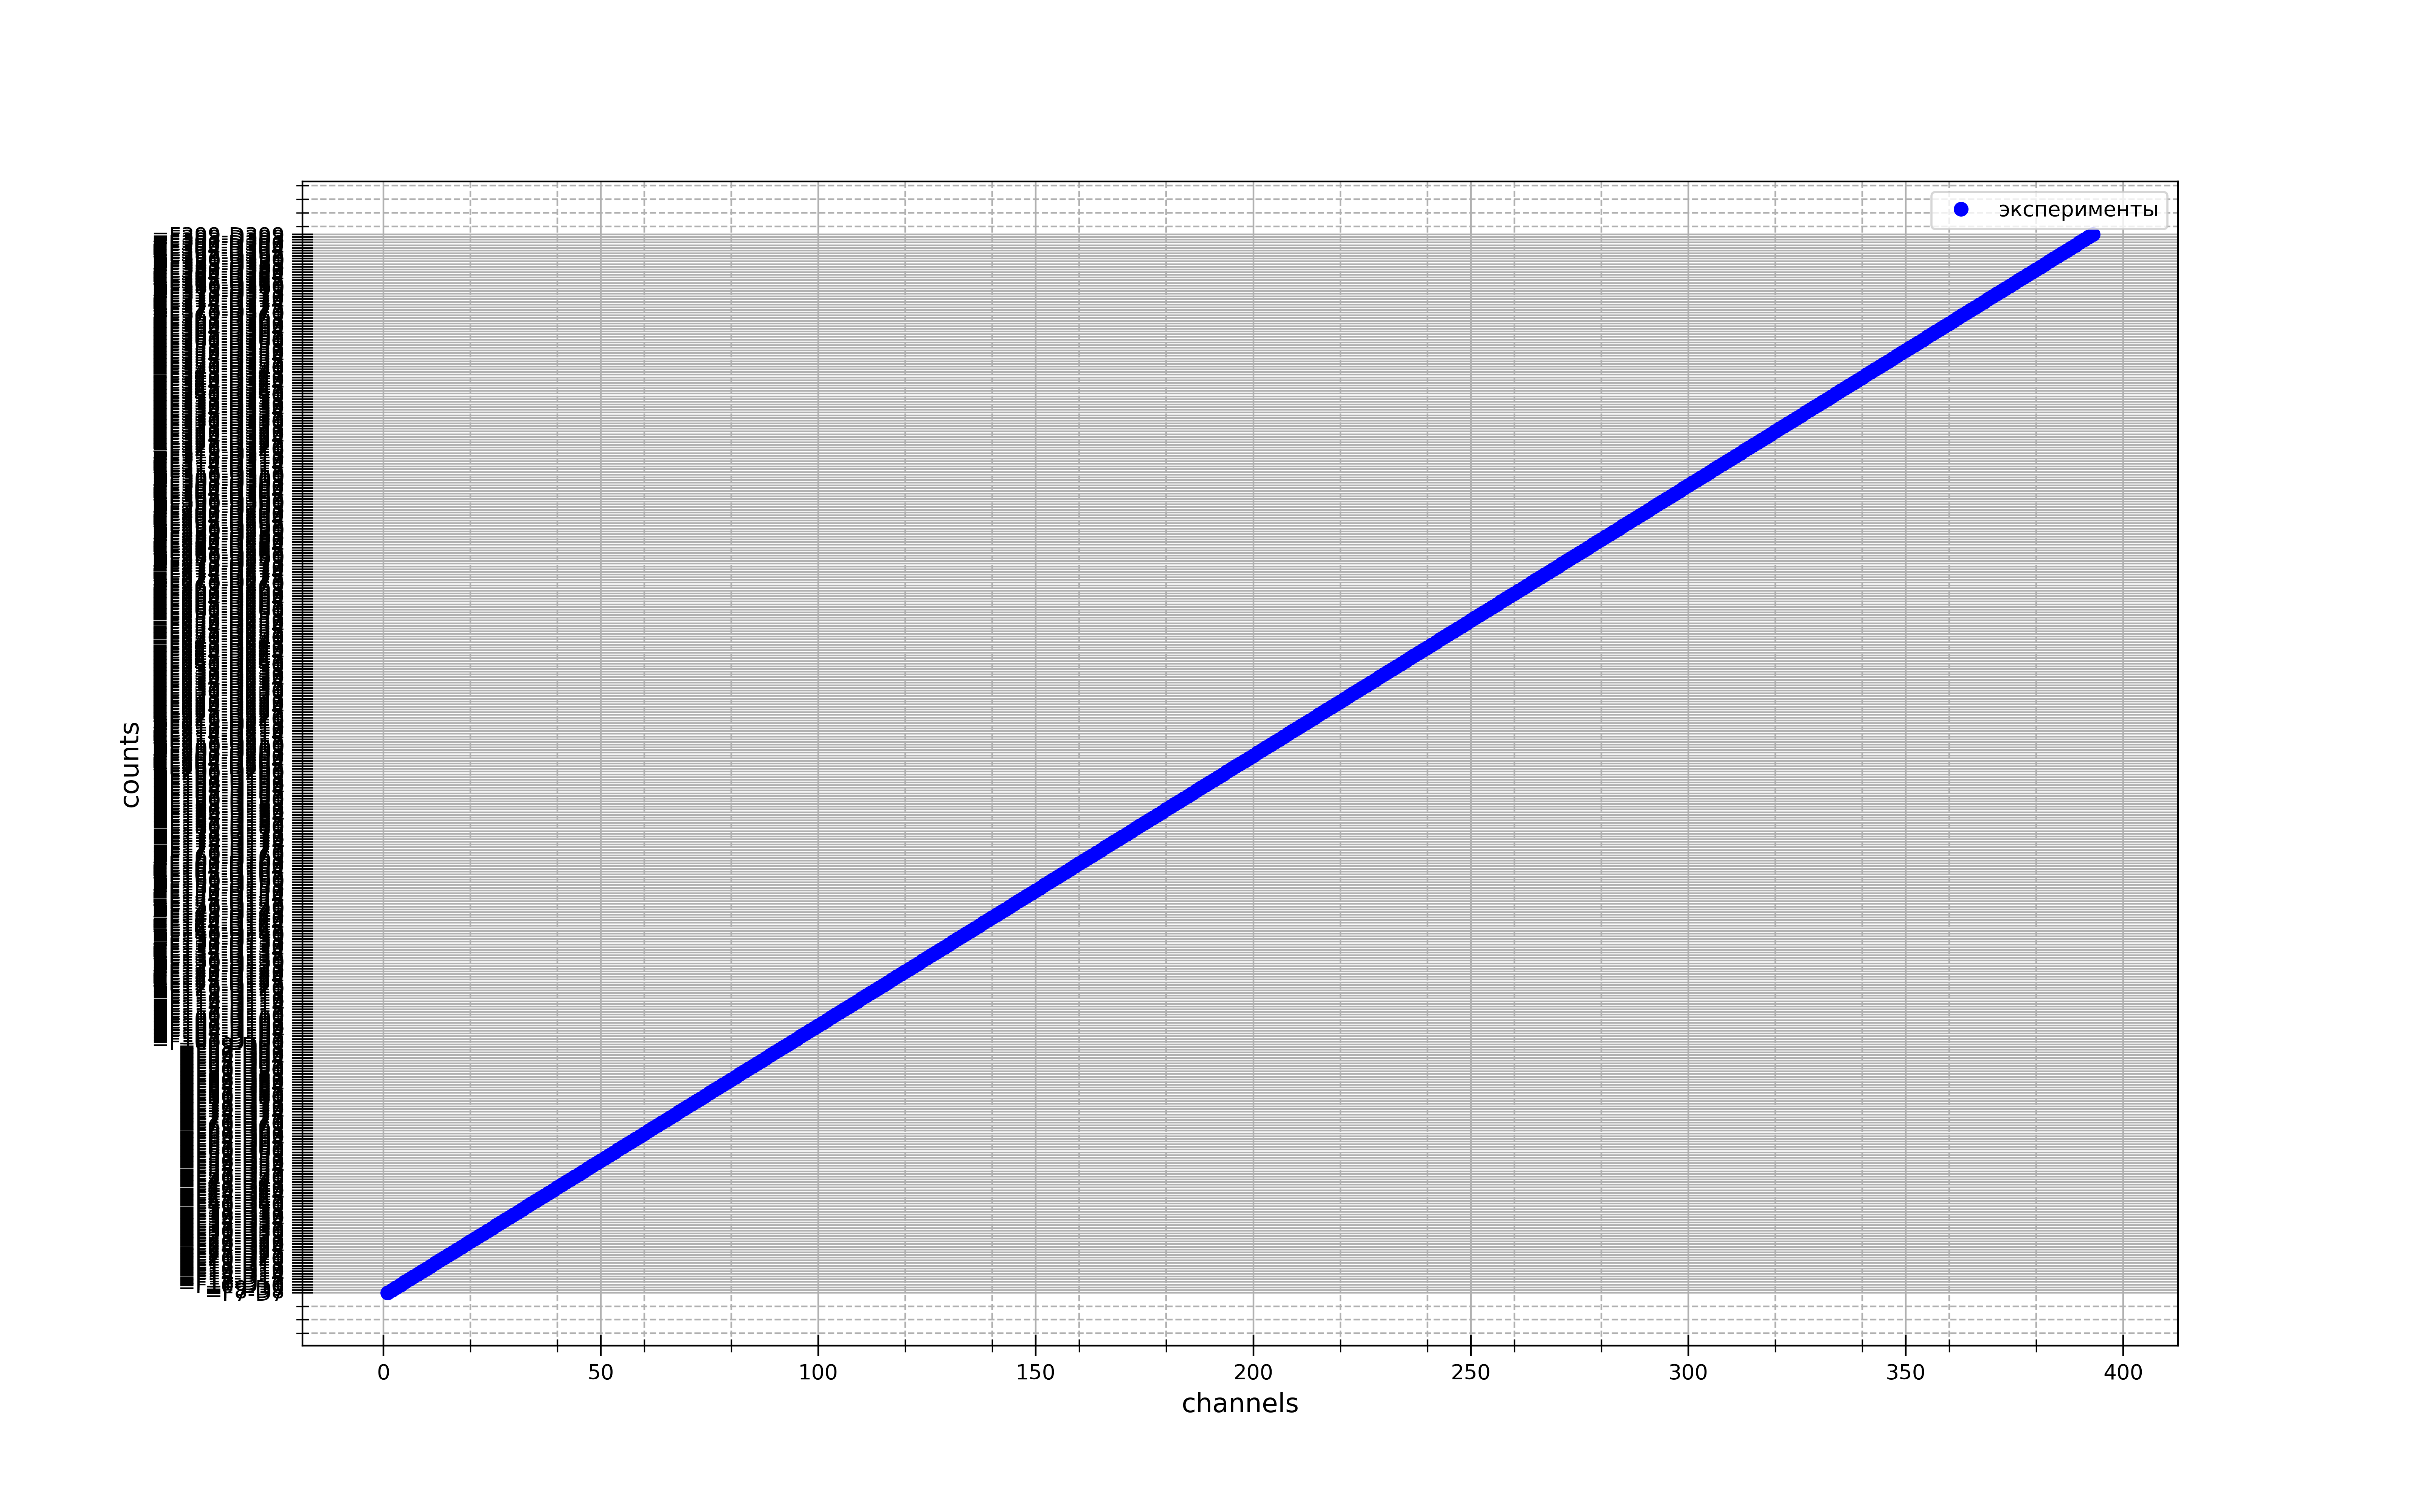
\includegraphics[width=0.8\linewidth]{na22-600.png}
\caption{Спектр $^{22}Na$}
\label{fig:mpr}
\end{figure}
\begin{figure}[!h]
\centering
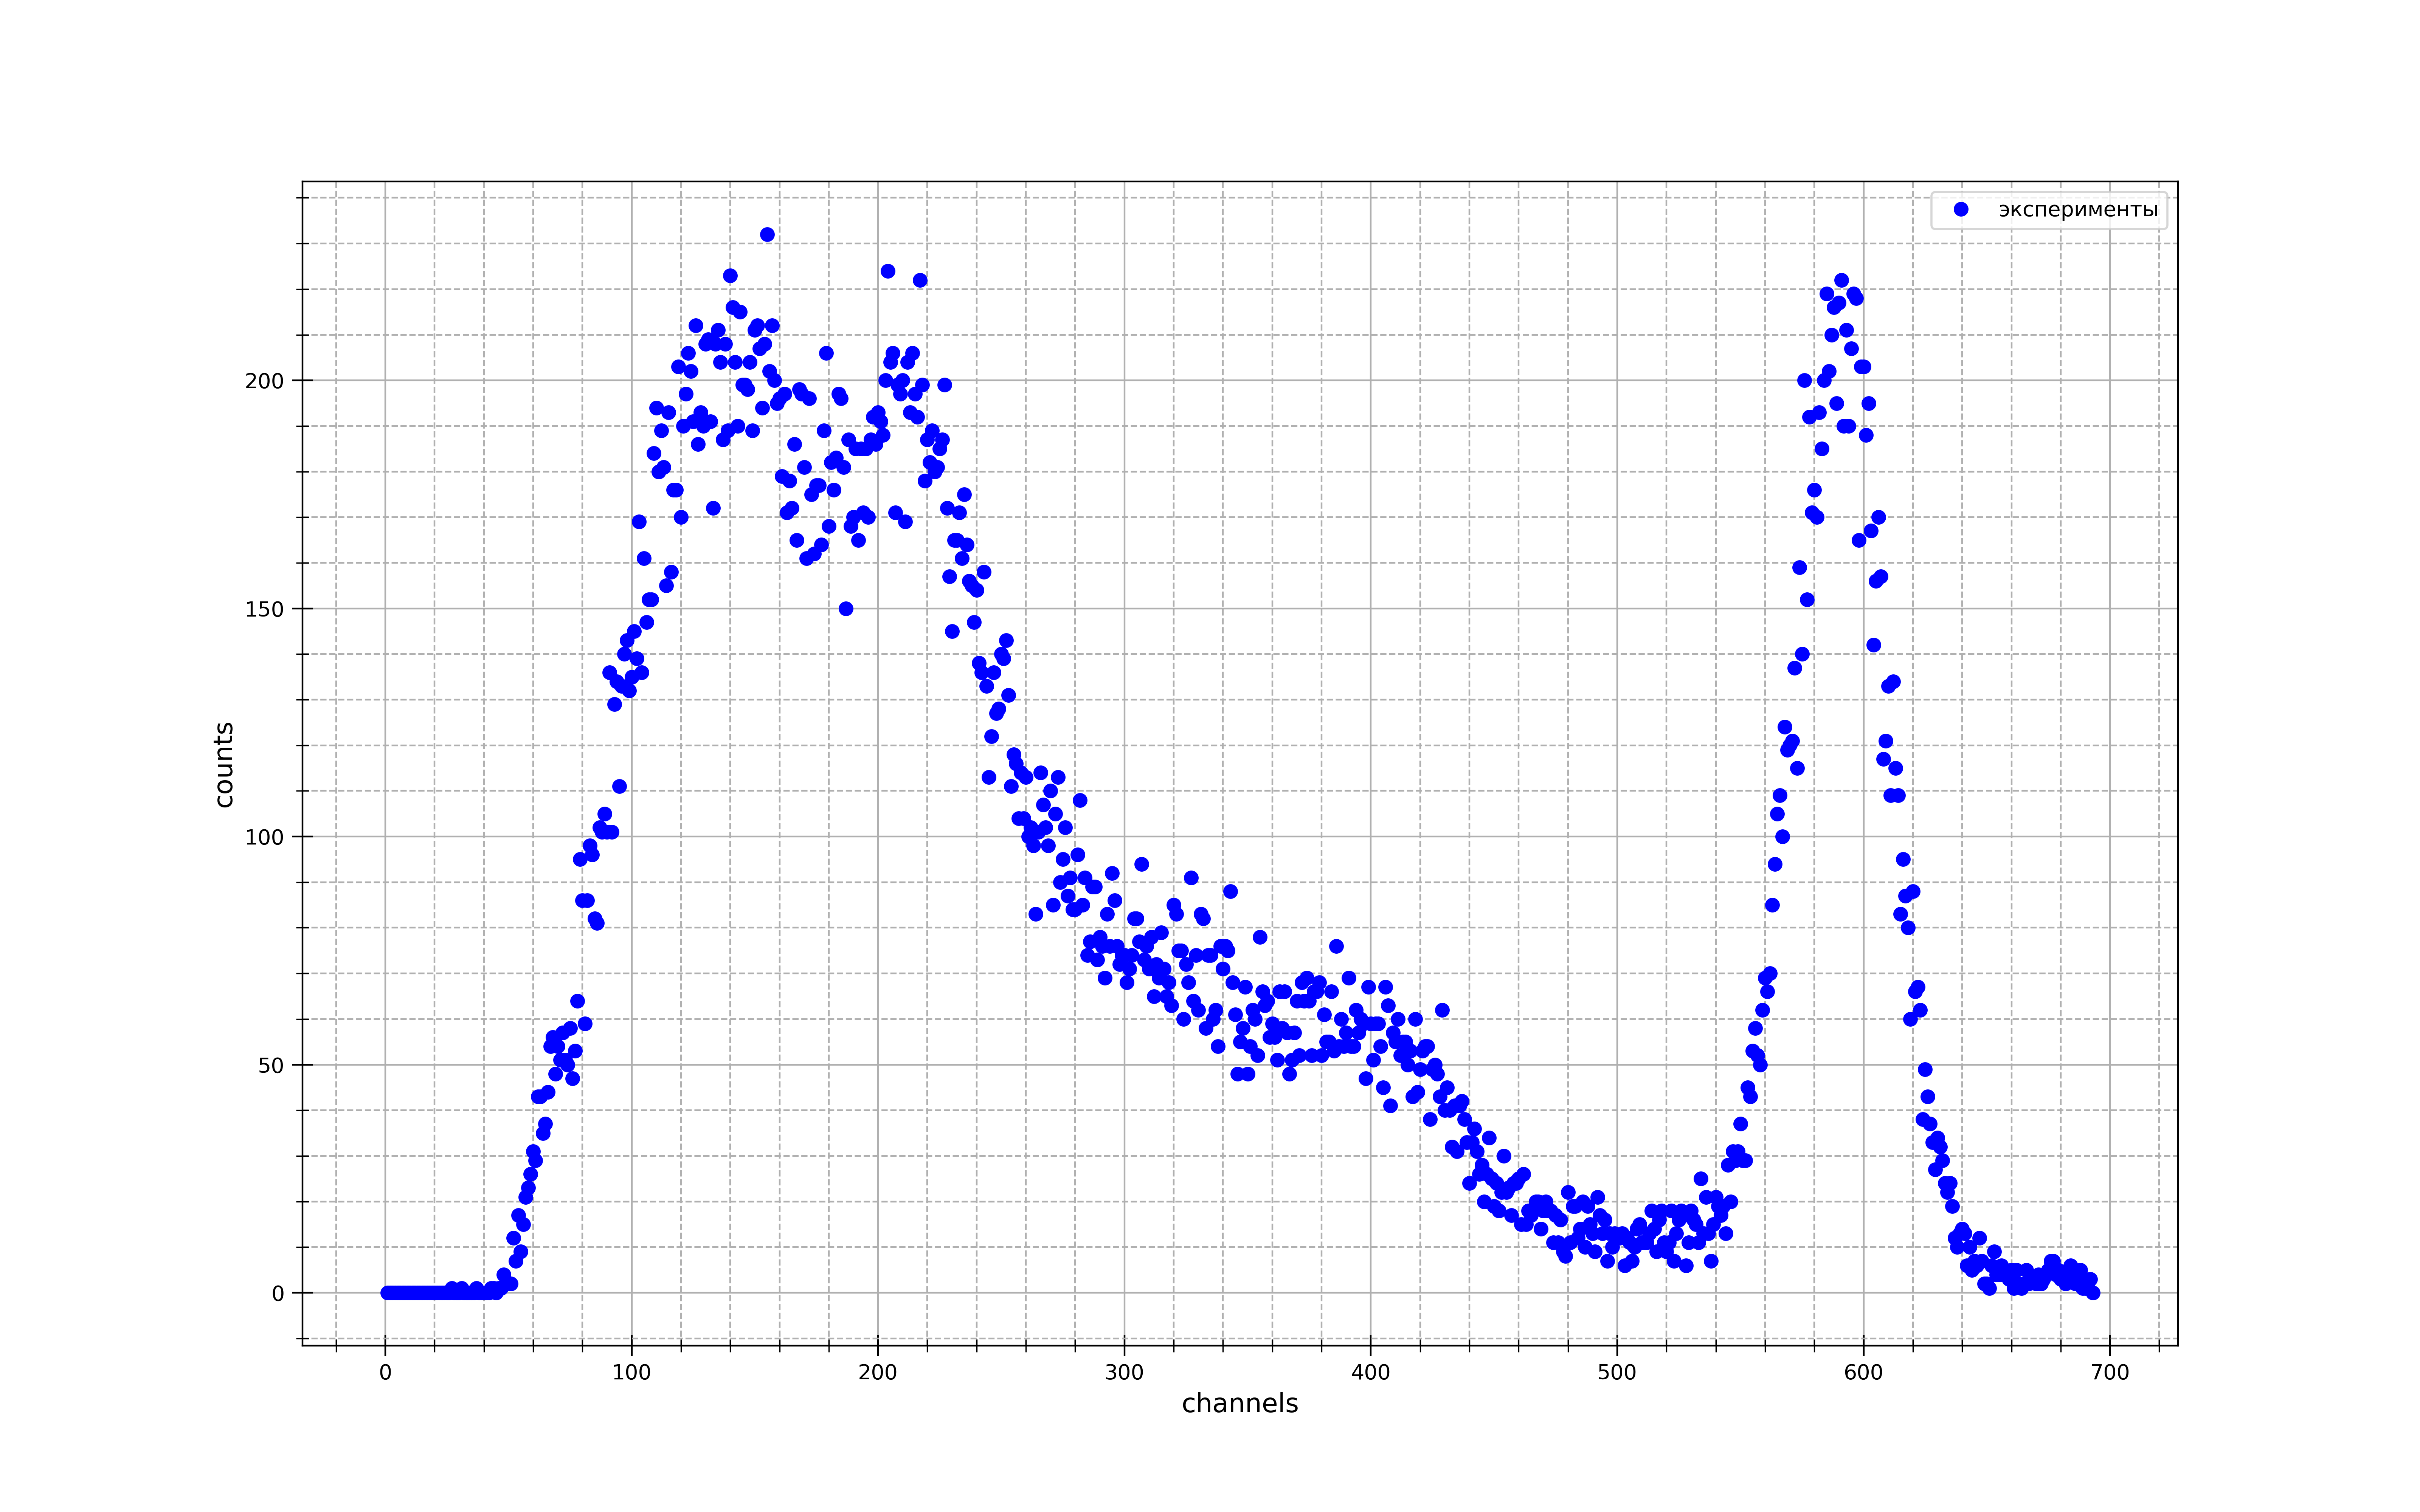
\includegraphics[width=0.8\linewidth]{cs137-600.png}
\caption{Спектр $^{137}Cs$}
\label{fig:mpr}
\end{figure}
\begin{figure}[!h]
\centering
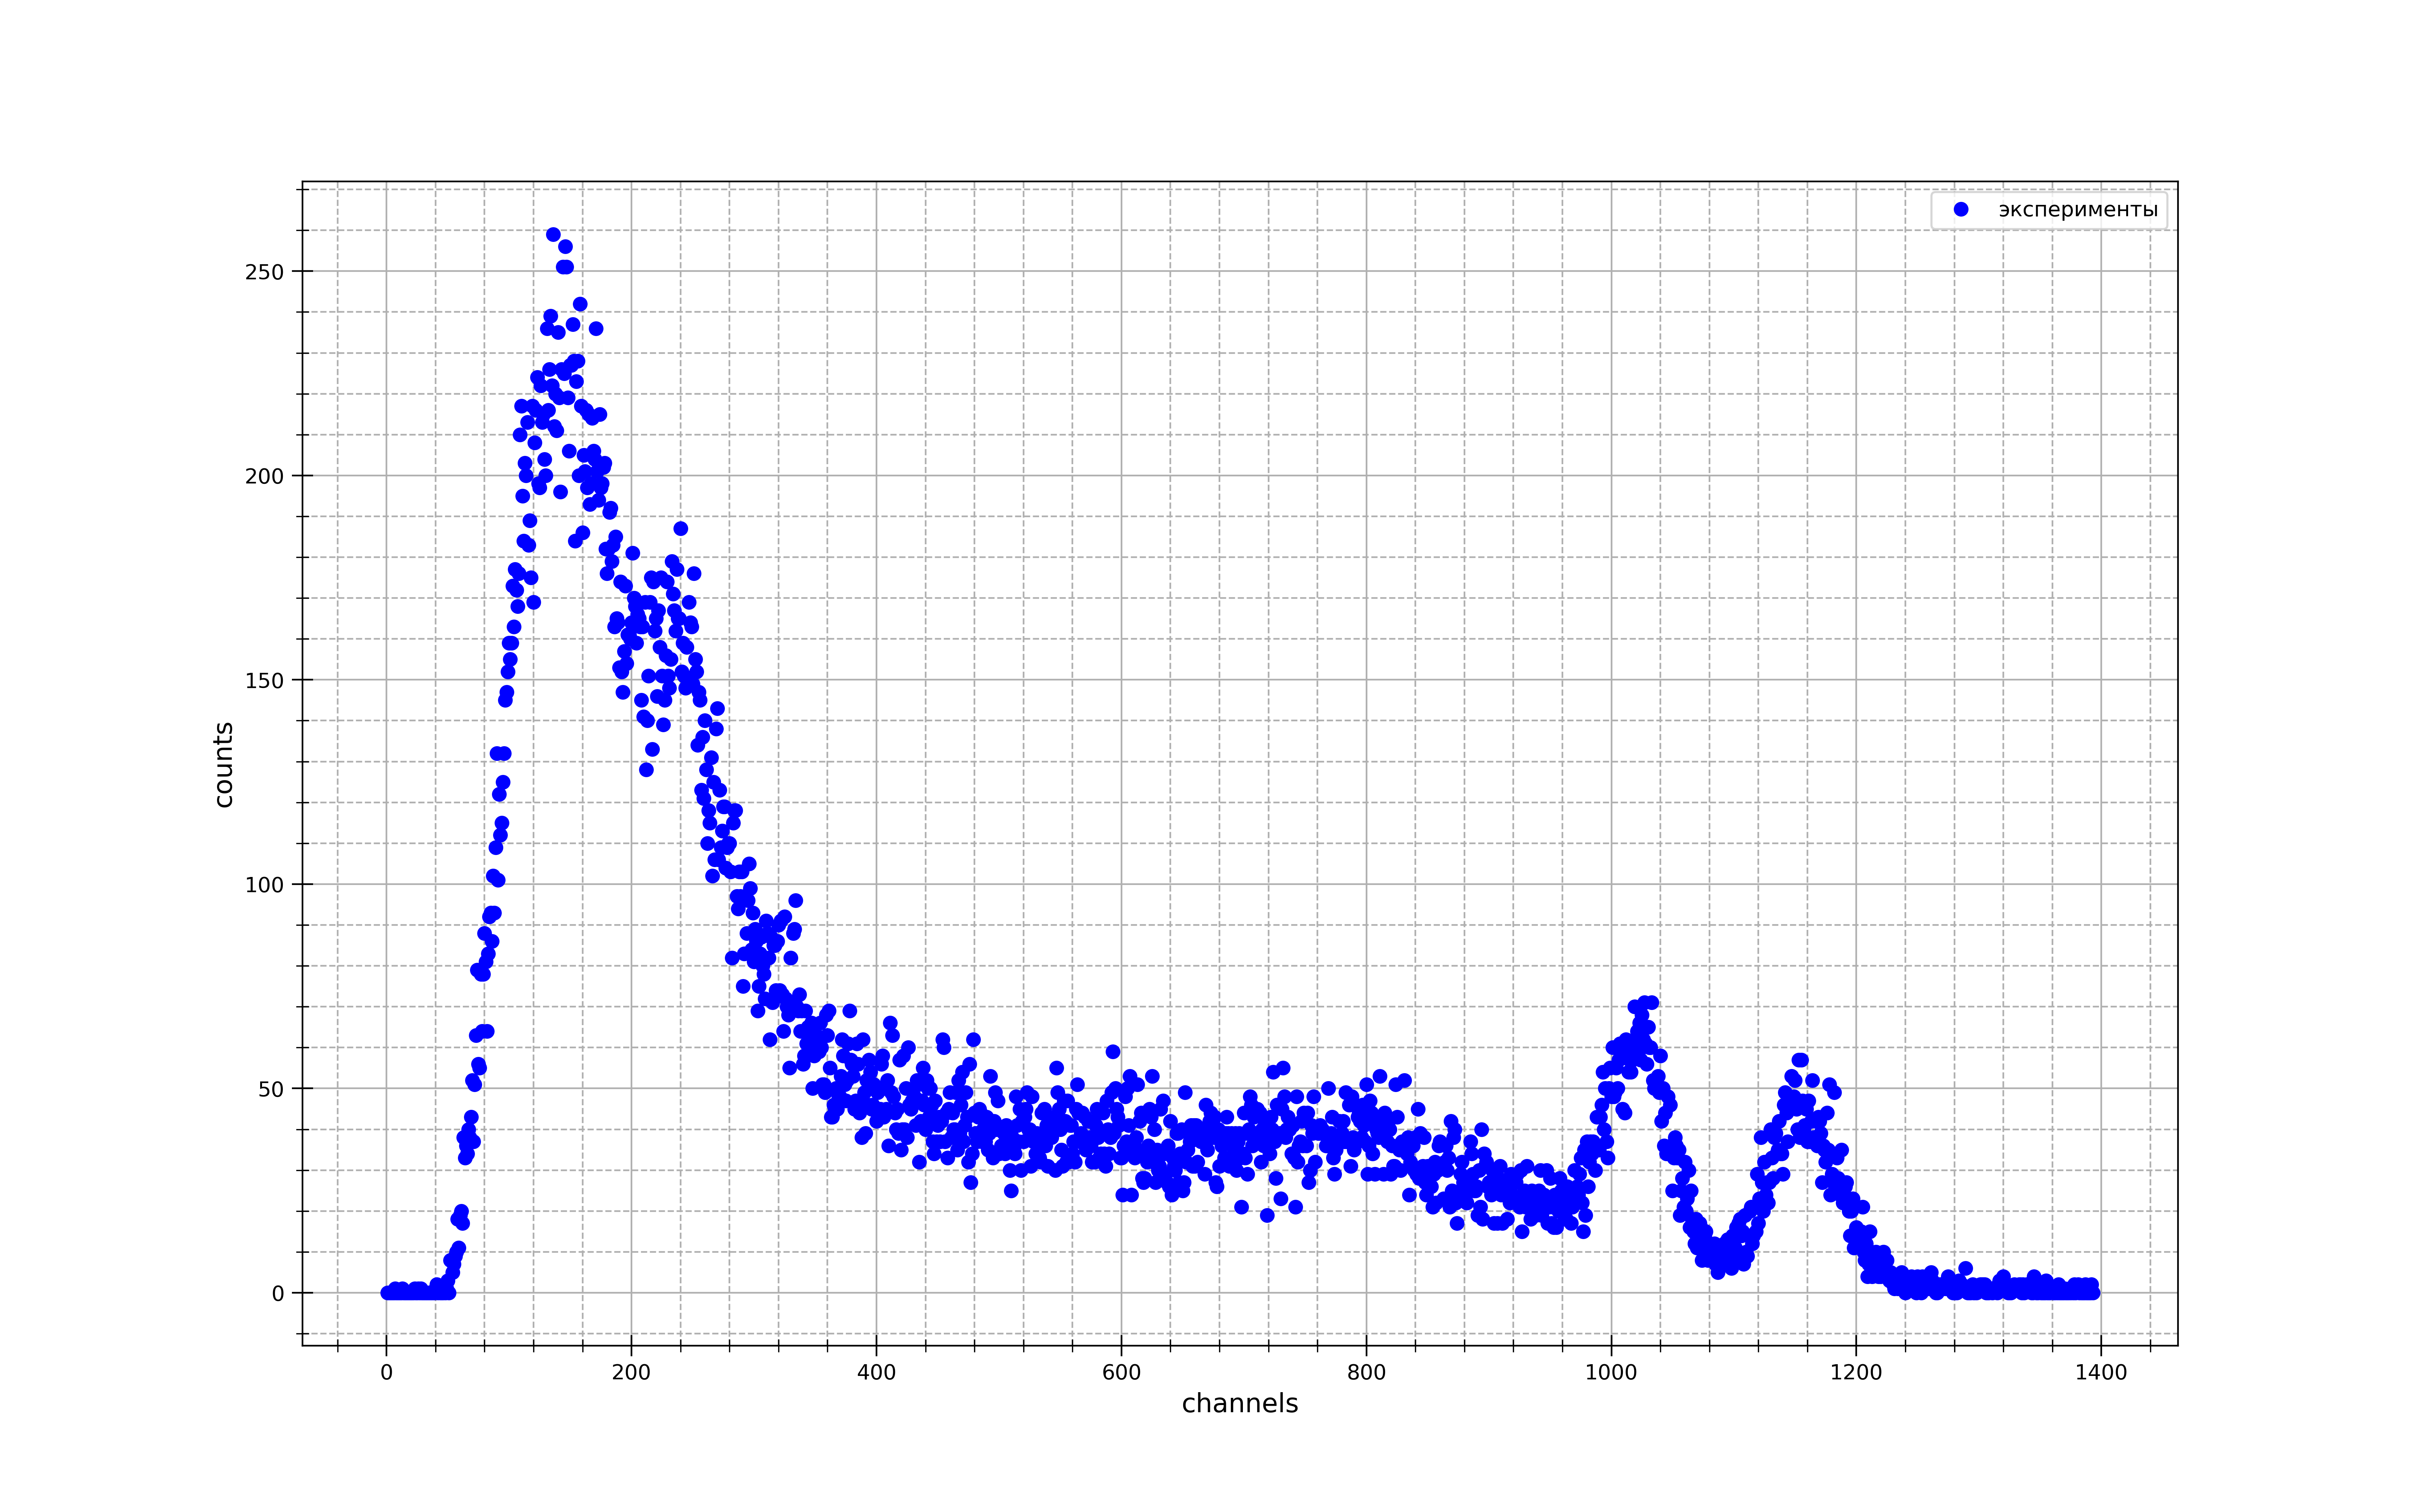
\includegraphics[width=0.8\linewidth]{co60-600.png}
\caption{Спектр $^{60}Co$}
\label{fig:mpr}
\end{figure}

\end{document}
